\documentclass[a4paper,11pt]{article}

\usepackage[utf8]{inputenc}
\usepackage[T1]{fontenc}
\usepackage{mathptmx}

\usepackage[a4paper,text={160mm,220mm},centering]{geometry}

\usepackage{hyperref}
\usepackage{listings}
\usepackage{graphicx}
\usepackage[table]{xcolor}

\lstset{basicstyle={\ttfamily}}

\usepackage{tikz}
\usepackage{pgf-pie}

\usepackage{todonotes}

\begin{document}

\thispagestyle{empty}

\unitlength=1mm
\begin{picture}(140,30)
\put(-10,30){\includegraphics[height=12mm]{../images/TIS-logo.png}}
\put(-10,11){
\includegraphics[height=22mm]{../images/adacore.png}}
\put(-6,0){
\includegraphics[height=12mm]{../images/logo_ocamlpro.png}}
\put(125,30){
\includegraphics[height=10mm]{../images/Universite_Paris_Saclay_logo.png}}
\put(127,12){
\includegraphics[height=16mm]{../images/cnrs.png}}
\put(123,0){
\includegraphics[height=12mm]{../images/logo-inria-reduced.png}}
\end{picture}

\vfill

\begin{center}

{ \Huge\bfseries
  Projet Décysif --- Livrable 1.1 }

\bigskip

{  \LARGE\bfseries
  Constitution d’une base de fichiers d’entrée
représentatifs des difficultés rencontrées pour
générer des exploits.
}

\vfill

\large Juillet 2024

\vfill

\large Guillaume Cluzel (TrustInSoft), Matteo Manighetti (Inria \& Université Paris-Saclay), Claude Marché
(Inria \& Université Paris-Saclay), Yannick Moy (AdaCore)

\end{center}

\vfill

\noindent\begin{picture}(140,30)
\put(0,0){
\includegraphics[width=0.3\textwidth]{../images/Logo_Bpifrance.png}}
\put(70,0){
\includegraphics[width=0.3\textwidth]{../images/LOGO_RIDF_2019_COULEUR.png}}
\put(145,0){
\includegraphics[width=0.1\textwidth]{../images/Logo-France-2030-rouge-bleu.png}}
\end{picture}

\noindent Le projet Décysif est financé par la Région Île-de-France et par le Gouvernement
Français dans le cadre du Plan France 2030

\clearpage

Ce livrable est constituée d'une base de tests qui se trouve dans le dépot
\href{https://github.com/Decysif/benchmarks}{'benchmarks'} du projet Décysif.

Objectifs du livrable :

\begin{itemize}
\item Repérer les faiblesses du prouveur Alt-Ergo
\item Repérer les problèmes de traduction (ou repérer des problèmes au
  niveau de l'écriture des théories, par exemple le modèle mémoire de
  J3) pour tous les prouveurs cvc5, CVC4, Z3, Alt-Ergo.
\item Identifier des faiblesses lors de la reconstruction d'un
  contre-exemple par Why3 depuis les modeles des solveurs
  SMT~\cite{dailler18jlamp}
\item Identifier les faiblesses des procédures de vérification et
  catégorisation des contre-exemples~\cite{becker21rr,becker21fide}
\end{itemize}

% Une section par répertoire d'exemples avec une description du contenu
% et de la méthodologie des statisques adoptée. Et le résultat de ces statisques
% au démarrage du projet.

% Mettre les statistiques qu'on a quand elles existent.

\section{Contre-Exemples générés sur du code  WhyML}

Le jeu de tests sur les contre-exemples en Why3 s'appuie sur
l'installation locale de Why3 qui est déjà décrite dans le livrable
2.1. Donc si ce n'est pas déjà fait, il faut installer et configurer Why3 en allant dans le répertoire \url{why3_exemple} et exécuter
\begin{lstlisting}
> ./import_suite.sh
\end{lstlisting}

\subsection{Suite de tests issues de Why3}

La suite de tests pour les contre-exemples se trouvent dans le
répertoire \url{why3_ce}. Il faut initialiser la suite de tests en
allant dans ce répertoire et exécuter
\begin{lstlisting}
> ./import_suite.sh
\end{lstlisting}
(il s'agit d'un autre script que le précédent)

Les tests peuvent ensuite être exécutés par la commande
\begin{lstlisting}
> ./run_bench.sh
\end{lstlisting}
Les résultats des tests sont stockés dans le sous-répertoire
\url{tests}. Des statistiques peuvent être calculées pour synthétiser
les résultats de ces tests, avec le script
\begin{lstlisting}
> ./ce-stats.py
\end{lstlisting}
qui génère des fichiers de statistiques au format CSV.

Une exécution de ces tests a été effectuée
le 22 avril 2024, avec les prouveurs Alt-Ergo 2.5.2, CVC4 1.8, cvc5
1.0.5 et Z3 4.8.10. les résultats globaux sont donnés par la table ci-dessous.
  \begin{center}
  \rowcolors{2}{gray!25}{white}
  \begin{tabular}{|l|r|r|}
    \hline
  \rowcolor{gray!50} Verdict
  & \multicolumn{1}{p{0.13\textwidth}|}{nombre d'occurrences}
  & \multicolumn{1}{p{0.13\textwidth}|}{pourcentage}
  \\
Non-Conformity (NC)         & 721 & 61,36 \% \\
Specification Weakness (SW) & 93 & 7,91 \% \\
NC or SW  	       & 6 & 0,51 \% \\
Bad Counterexample (BAD) & 195 & 16,60 \% \\
    Validation Incompleteness (INC) & 160 & 13,62 \% \\
    \hline
  \end{tabular}
\end{center}
Ces statistiques sont également visualisées par le diagramme
  suivant.
  \begin{center}
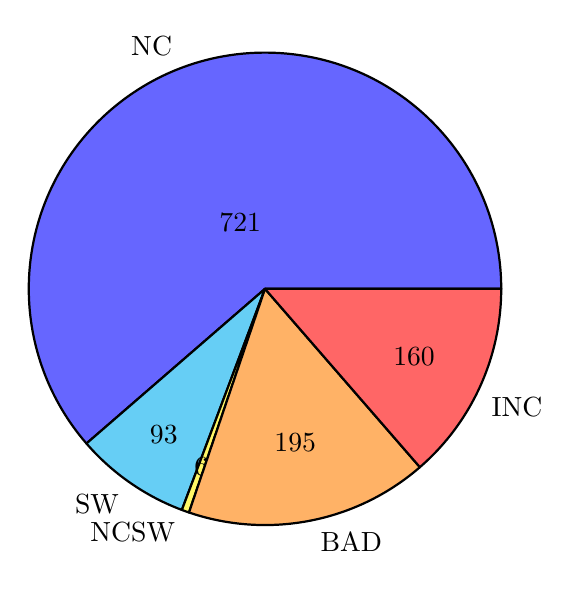
\begin{tikzpicture}
    \pie[sum=auto]{721/NC, 93/SW, 6/NCSW, 195/BAD, 160/INC}
\end{tikzpicture}
\end{center}
La première ligne «~Non-Conformity~» (en abrégé NC) désigne les cas où une
erreur de code à été effectivement identifiée, plus précisément un cas où le
code n'est pas conforme à la spécification, et où un contre-exemple explicite
est produit pour générer l'exploit correspondant. La seconde ligne
«~Specification Weakness~» (SW) concerne les cas où un contre-exemple est généré
mais qui ne révèle pas un exploit mais une insuffisance dans les spécifications
(manque d'invariant de boucle où sous-spécification d'une fonction auxiliaire)
qui empêche de faire une preuve. Ces deux cas sont des cas favorables, et on va
chercher à augmenter leurs fréquences. Le cas «~NC or SW~» désigne les cas où l'on
n'arrive pas à décider si le contre-exemple est un exploit ou bien si c'est une
faiblesse de spécification. C'est aussi une situation favorable mais plus
imprécise. le cas «~Bad Counterexample~» (BAD) est défavorable : le contre-exemple
proposé par le solveur n'est en fait pas un bon contre-exemple, et ce fait a été
détecté comme tel par la procédure de validation. On souhaite diminuer le
pourcentage de ces cas, et la seule façon que l'on a pour réduire ce pourcentage
est de modifier les tâches de preuve que l'on soumet au solveur, afin que
celui-ci soit plus performant. Le dernier cas «~Validation Incompleteness~»
(INC) est aussi défavorable et on va chercher à le diminuer. Pour cela, il faut
jouer sur la méthodologie actuelle pour valider les contre-exemples, telle
qu'implémentée dans Why3.  Le taux de cas favorables est de l'ordre de 70\%, et
l'augmentation de ce taux est donc un objectif général.

Pour le dernier cas «~Validation Incompleteness~», on peut donner des
statistiques plus détaillées. Voici ces statistiques pour la partie de
validation dite «~à petits pas~» (cf~\cite{becker21fide})
  \begin{center}
  \rowcolors{2}{gray!25}{white}
  \begin{tabular}{|l|r|r|}
    \hline
    \rowcolor{gray!50} Réponse
  & \multicolumn{1}{p{0.65\textwidth}|}{explication}
  & \multicolumn{1}{p{0.13\textwidth}|}{nombre d'occurrences}
    \\
INCOMPLETE & cannot decide	& 127 \\
INCOMPLETE & missing return value & 11 \\
INCOMPLETE & uncaught exception	& 8 \\
INCOMPLETE & (terminated because mlmpfr wrapper is not implemented) & 6 \\
INCOMPLETE & many args for exec	& 2 \\
INCOMPLETE & (terminated because index is out of bounds) & 1 \\
    INCOMPLETE & (terminated because missing value for global `get`) & 1 \\
    \hline
\end{tabular}
\end{center}
Les deux premières lignes correspondent à des améliorations à apporter
à la méthodologie. Les autres lignes correspondent a priori tout
simplement à des bugs qu'il faut corriger.

Les statistiques pour la
partie de validation dite «~à pas de géant~»~\cite{becker21rr} sont les suivantes.
\begin{center}
  \rowcolors{2}{gray!25}{white}
  \begin{tabular}{|l|r|r|}
    \hline
  \rowcolor{gray!50} Réponse
  & \multicolumn{1}{p{0.65\textwidth}|}{explication}
  & \multicolumn{1}{p{0.13\textwidth}|}{nombre d'occurrences}
    \\
INCOMPLETE & cannot decide	& 129 \\
INCOMPLETE & missing return value  &	15 \\
INCOMPLETE & uncaught exception	& 8 \\
INCOMPLETE &  (terminated because mlmpfr wrapper is not implemented) &	6 \\
INCOMPLETE & (terminated because index is out of bounds) &	1 \\
    INCOMPLETE & (terminated because missing value for global `get`) &	1 \\
    \hline
  \end{tabular}
\end{center}
Les conclusions sont les mêmes que pour la partie petits pas: deux
pistes d'amélioration, et des bugs à corriger.


\subsection{Suite de tests construits à la main}

Une autre base de tests est construite manuellement dans l'objectif d'améliorer
la façon de présenter un contre-exemple. Cette restitution est importante pour
un utilisateur de Why3 mais aussi pour les différents front-end pour le C ou
pour Ada. Ce jeu de tests est donné dans le sous-répertoire \url{tests_for_log}
du répertoire \url{why3_ce}. Pour ces tests, on ne mesure pas leur succès par des
statistiques mais par une proximité avec un résultat attendu. Les résultats
attendus pour ces tests seront décrits dans un livrable annexe à celui-ci d'ici
la fin 2024 au plus tard.  \footnote{Les sources de cette annexe sont
  actuellement dans le sous-répertoire \url{counterexamples} du dépôt
  \url{livrables}}

\section{Contre-Exemples issus de J3}

Le répertoire \url{j3_ce} contient une suite de tests au format C qui peuvent
être rejoués en utilisant tis-analyzer, comme expliqué dans le fichier
\url{README.md} de ce répertoire. En particulier, le répertoire contient
deux scripts~: le premier permettant de générer des fichiers au format
\texttt{sexp} pouvant être réutilisés ultérieurement par un utilisateur n'ayant
pas installé tis-analyzer, et un second script permettant de lancer la suite
de tests et obtenir des statisques sur les contres-exemples de la suite de tests.

Une exécution de ces tests a été effectuée le 21 juin 2024 en utilisant la
version 1.47 de tis-analyzer, utilisant les prouveurs CVC4 1.7, cvc5 1.0.5 et
Z3 4.8.17. Les résultats globaux de la classification de ces contre-exemples
sont donnés ci-dessous.

\begin{center}
  \rowcolors{2}{gray!25}{white}
  \begin{tabular}{|l|r|r|}
    \hline
  \rowcolor{gray!50} Verdict
  & \multicolumn{1}{p{0.13\textwidth}|}{nombre d'occurrences}
  & \multicolumn{1}{p{0.13\textwidth}|}{pourcentage}
  \\
Non-Conformity (NC)                 & 147 & 70 \% \\
Specification Weakness (SW)         &  14 &  7 \% \\
NC or SW  	                        &  31 & 15 \% \\
Bad Counterexample (BAD)            &   3 &  1 \% \\
    Validation Incompleteness (INC) &  15 &  7 \% \\
    \hline
  \end{tabular}
\end{center}
Ces statistiques sont également visualisées par le diagramme
suivant.
  \begin{center}
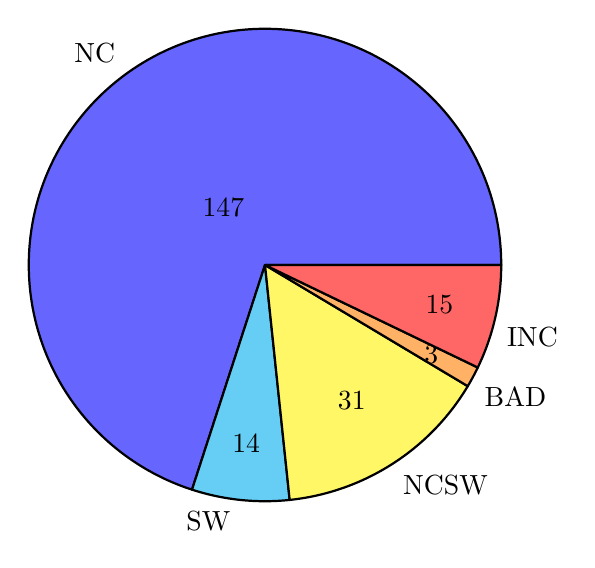
\begin{tikzpicture}
    \pie[sum=auto]{147/NC, 14/SW, 31/NCSW, 3/BAD, 15/INC}
\end{tikzpicture}
\end{center}

La classification des contre-exemples dans J3 se fait à l'aide de deux outils
indépendants de J3. Le premier de ces deux outils est le greffon d'analyse par
interpretation abstraite de tis-analyzer qui est utilisé en mode «~interpréteur~»
ce qui représente une exécution concrète du source C. Cette partie étant assez
stable et ses limitations déjà identifiées, le choix a été fait de se concentrer
sur l'extration de statistiques autour du deuxième outil permettant la
classification des contre-exemples. Cet outil est l'interpréteur de code dit
«~à pas de géant~». Les résultats de l'interpréteur de code «~à pas de géant~»
sont donnés dans la table ci-dessous.

\begin{center}
  \rowcolors{2}{gray!25}{white}
  \begin{tabular}{|l|r|r|}
    \hline
  \rowcolor{gray!50} Verdict
  & \multicolumn{1}{p{0.13\textwidth}|}{nombre d'occurrences}
  & \multicolumn{1}{p{0.13\textwidth}|}{pourcentage}
  \\
    NORMAL                              &  20 &  4 \% \\
    FAILURE                             & 294 & 63 \% \\
    STUCK                               &  36 &  8 \% \\
    INCOMPLETE                          & 111 & 24 \% \\
    \hline
  \end{tabular}
\end{center}

La ligne «~STUCK~» révèle des problèmes dans l'exécution à pas de géant du
contre-exemple. C'est un cas défavorable qui empêche d'évaluer la qualité
du contre-exemple et empêche également de le classifier.
On cherche à isoler ces cas pour en réduire le pourcentage.
Le cas «~INCOMPLETE~» rélève lui aussi des problèmes dans l'évaluation de
la validité du contre-exemple retourné par le prouveur. Les raisons
peuvent être diverses, et les analyser permettra de classer correctement plus
de contre-exemples.
La ligne «~NORMAL~» correspond à un modèle retourné par le prouveur qui ne
viole aucune contrainte du code. Ces cas seront analysés pour comprendre
pourquoi le proveur a retourné des modèles qui ne constitue pas un
contre-exemple pour la propriété que l'on cherche à prouver et permettra de
déterminer les leviés possibles pour l'amélioration des contre-exemples dans J3.
Enfin, la ligne «~FAILURE~» correspond au cas d'un contre-exemple correct, c'est
donc le cas favorable. L'objectif général est d'augmenter le taux
de contre-exemples classé dans cette dernière catégorie et de diminuer les
taux des trois autres catégories.

\section{Contre-Exemples issus de SPARK}

\subsection{Résultats sur la suite complète de tests de SPARK}

Comme indiqué dans le fichier \url{README.md} du répertoire \url{spark_ce}, il est
possible en utilisant l'environnement de tests d'AdaCore de générer des
informations sur la qualité des contre-exemples générés pour la suite complète
des tests de SPARK. Comme pour Why3, nous pouvons générer des fichiers de
statistiques au format CSV.

Une exécution de ces tests a été effectuée le 5 juin 2024, avec le prouveur cvc5
1.0.5 pour générer des contre-exemples. Les résultats globaux sont donnés par la
table ci-dessous.

\begin{center}
  \rowcolors{2}{gray!25}{white}
  \begin{tabular}{|l|r|r|}
    \hline
  \rowcolor{gray!50} Verdict
  & \multicolumn{1}{p{0.13\textwidth}|}{nombre d'occurrences}
  & \multicolumn{1}{p{0.13\textwidth}|}{pourcentage}
  \\
Non-Conformity (NC)            & 1199 & 23 \% \\
Specification Weakness (SW)    &  153 &  3 \% \\
NC or SW  	          &  819 & 16 \% \\
Bad Counterexample (BAD)       &  592 & 11 \% \\
    Validation Incompleteness (INC) & 2465 & 47 \% \\
    \hline
  \end{tabular}
\end{center}
Ces statistiques sont également visualisées par le diagramme
suivant.
  \begin{center}
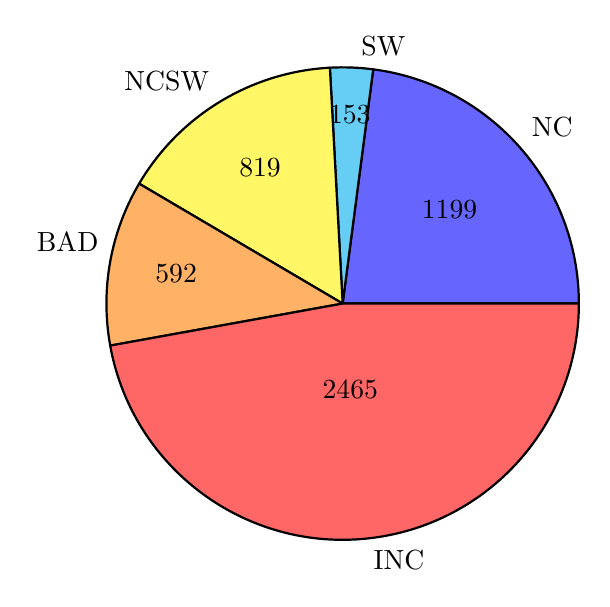
\begin{tikzpicture}
    \pie[sum=auto]{1199/NC, 153/SW, 819/NCSW, 592/BAD, 2465/INC}
\end{tikzpicture}
\end{center}

Par rapport aux résultats rapportés pour Why3, les cas favorables
(Non-Conformity + Specification Weakness + NC or SW) représentent une plus
faible proportion du nombre total des contre-exemples générés de seulement 42\%,
que l'on cherche donc à augmenter.

Pour le dernier cas «~Validation Incompleteness~», on peut donner des
statistiques plus détaillées. Voici ces statistiques pour la partie de
validation dite «~à petits pas~» :

\begin{center}
  \rowcolors{2}{gray!25}{white}
  \begin{tabular}{|l|r|r|}
  \hline
  \rowcolor{gray!50} Réponse
  & \multicolumn{1}{p{0.65\textwidth}|}{explication}
  & \multicolumn{1}{p{0.13\textwidth}|}{nombre d'occurrences}
    \\
INCOMPLETE & unsupported                             & 1231 \\
INCOMPLETE & no body                                 &  455 \\
INCOMPLETE & missing parameter value                 &  402 \\
INCOMPLETE & normal                                  &  251 \\
INCOMPLETE & no subprogram body	                     &   38 \\
INCOMPLETE & no VC                                   &   36 \\
INCOMPLETE & out of fuel                             &   36 \\
INCOMPLETE & expr with private type                  &   10 \\
INCOMPLETE & protected component or part of variable &    4 \\
    INCOMPLETE & no reason                               &    2 \\
    \hline
\end{tabular}
\end{center}

La première ligne, qui représente la moitié des cas d'incomplétude, correspond à
tous les cas qui ne sont pas encore traités dans la validation à petits pas, qui
est réalisée par un interpréteur de code Ada dédié, c.-à-d. programmé
spécifiquement pour cet usage. C'est un axe important d'amélioration pour le
futur.

Les lignes «~no body~» et «~no subprogram body~» représentent les cas où
l'implémentation d'un sous-programme n'est soit pas disponible (à cause de la
façon dont l'outil de validation aggrège le code) ou bien pas en SPARK (ce qui
empêche aujourd'hui la validation qui n'a aujourd'hui été implémentée que
pour les constructions SPARK). La ligne «~missing
parameter value~» représente les cas où aucune valeur n'est disponible pour une
variable du programme.

La ligne «~normal~» correspond aux cas où la validation à petits pas s'exécute
sans erreur alors que la validation dite «~à pas de géant~» est incomplète. Il faut
dans ce cas examiner les raisons de cette autre source d'incomplétude.

Nous ne détaillons pas plus les cas correspondants aux lignes restantes qui
concernent beaucoup moins de contre-exemples.

Les statistiques pour la
partie de validation dite «~à pas de géant~» sont les suivantes.
\begin{center}
  \rowcolors{2}{gray!25}{white}
  \begin{tabular}{|l|r|r|}
    \hline
  \rowcolor{gray!50} Réponse
  & \multicolumn{1}{p{0.65\textwidth}|}{explication}
  & \multicolumn{1}{p{0.13\textwidth}|}{nombre d'occurrences}
    \\
INCOMPLETE & cannot decide	   & 1754 \\
INCOMPLETE & no reason             &  259 \\
    INCOMPLETE & missing return value  &  151 \\
    \hline
  \end{tabular}
\end{center}
Les conclusions sont les mêmes que pour la validation des contre-exemples en
Why3 avec deux pistes d'amélioration, et des cas (``no reason'') pour laquelle
une investigation plus poussée est nécessaire.

\subsection{Suite de tests issue de SPARK}

La suite de tests réduite pour les contre-exemples se trouvent dans l'archive
\url{spark_sexp.zip} du répertoire \url{spark_ce}.  Le code archivé correspond
au code Why3 extrait par l'exécution de gnatprove sur le code SPARK d'une liste de
26 tests spécialement sélectionnés pour leur valeur pour les contre-exemples
(listés dans le fichier \url{MANIFEST.bench}). Pour installer et configurer ce
jeu de tests, les commandes
\begin{lstlisting}
> unzip spark_sexp.zip
> export PATH=$PWD/../why3_examples/why3-88dc033/bin:$PATH
> ./build_environment.sh
> make
\end{lstlisting}
doivent être exécutées au préalable. Cela suppose que le setup dans \url{why3_examples}
a été effectué au préalable afin de récupèrer une version de
référence de Why3 (1er mars 2024) et de compiler les commandes nécessaires. Ensuite la commande
\begin{lstlisting}
> ./run_bench.sh
\end{lstlisting}
doit être lancée pour exécuter les tests proprement dit.

Une execution du jeu de test a eu lieu le 25 juin 2024, avec le prouveur cvc5 dans
la configuration de Why3 ainsi que dans celle de SPARK (alternative "gnatprove").
Le résultats ont été les suivants:

\begin{center}
  \rowcolors{2}{gray!25}{white}
  \begin{tabular}{|l|r|r|r|}
    \hline
  \rowcolor{gray!50} Prouveur
  & \multicolumn{1}{p{0.4\textwidth}|}{Verdict}
  & \multicolumn{1}{p{0.13\textwidth}|}{nombre d'occurrences}
  & \multicolumn{1}{p{0.13\textwidth}|}{pourcentage} \\
cvc5,1.0.5,counterexamples & NC         & 68 & 0,22\\
cvc5,1.0.5,counterexamples & SW         & 0 & 0\\
cvc5,1.0.5,counterexamples & NC or SW   & 126& 0,42\\
cvc5,1.0.5,counterexamples & INCOMPLETE & 90 & 0,30\\
cvc5,1.0.5,counterexamples & BAD        & 17 & 0,06\\
    \hline
cvc5,1.0.5,gnatprove       & NC         & 68 & 0,22\\
cvc5,1.0.5,gnatprove       & SW         & 0 & 0\\
cvc5,1.0.5,gnatprove       & NC or SW   & 126& 0,42\\
cvc5,1.0.5,gnatprove       & INCOMPLETE & 84 & 0,28\\
cvc5,1.0.5,gnatprove       & BAD        & 24 & 0,08\\
    \hline
  \end{tabular}
\end{center}

Les statistiques pour la configuration gnatprove sont également visualisées par
le diagramme suivant.
\begin{center}
  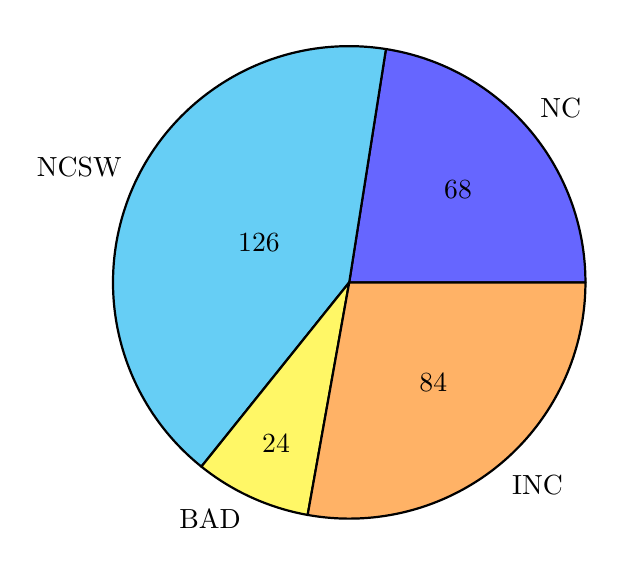
\begin{tikzpicture}
    \pie[sum=auto]{68/NC, 126/NCSW, 24/BAD, 84/INC}
  \end{tikzpicture}
\end{center}

L'execution à petits pas est maintenant executée par Why3, et non sur le code
Ada: c'est une raison possible pour le nombre plus faible de cas d'incompletude.
En plus, SPARK ne fournit pas le corp des sous-programmes, ce qui est nécessaire
pour reconnaître les cas SW.

Le detail de cas d'incompletude pour l'execution à petits pas est le suivant:

\begin{center}
  \rowcolors{2}{gray!25}{white}
  \begin{tabular}{|l|r|r|}
    \hline
  \rowcolor{gray!50} Réponse
  & \multicolumn{1}{p{0.65\textwidth}|}{explication}
  & \multicolumn{1}{p{0.13\textwidth}|}{nombre d'occurrences}
    \\
INCOMPLETE & cannot decide & 42 \\
INCOMPLETE & missing return value & 33 \\
INCOMPLETE & (terminated because RAC timelimit reached) & 9 \\
    \hline
  \end{tabular}
\end{center}

On peut voir qu'il ne s'agit pas de bug dans Why3, mais de cas qui nécessitent
des améliorations dans la méthodologie de validation des contre-exemples.

Le détail de l'execution à pas de géant est le suivant:

\begin{center}
  \rowcolors{2}{gray!25}{white}
  \begin{tabular}{|l|r|r|}
    \hline
  \rowcolor{gray!50} Réponse
  & \multicolumn{1}{p{0.65\textwidth}|}{explication}
  & \multicolumn{1}{p{0.13\textwidth}|}{nombre d'occurrences}
    \\
INCOMPLETE & cannot decide & 52 \\
NORMAL & & 19 \\
INCOMPLETE & missing return value & 8 \\
INCOMPLETE & (terminated because RAC timelimit reached) & 5 \\
    \hline
  \end{tabular}
\end{center}

Ici, on a un certain nombre de cas normaux, qui sont des modèles fourni par le
prouveur qui ne sont pas des contre-exemples.

\section{Travail futur}

Quelles autres statistiques peut-on vouloir? plus de détail sur les cas ``cannot decide'' ?

Futur: extraire depuis les contre-exemples classifiés comme NC des
exploits. Peut-etre un besoin d'indentifier des exemples dédiés sur lesquels on
sait que des exploits existent, et on veut montrer que l'on sait les identifier.

Un travail futur est également de créer une infrastructure de production de
contre-exemples pour Creusot~\cite{denis22icfem}.

\clearpage

\bibliographystyle{plainurl}
\bibliography{generated,main}
%\bibliography{abbrevs,demons,demons2,demons3,team,crossrefs}

\end{document}


% Local Variables:
% mode: latex
% mode: flyspell
% TeX-master: t
% TeX-PDF-mode: t
% ispell-local-dictionary: "francais"
% fill-column: 80
% End:
